\documentclass[11pt,a4paper]{article}
\usepackage[utf8]{inputenc}
\usepackage[T1]{fontenc}
\usepackage[spanish,es-noindentfirst]{babel}
\usepackage{graphicx}
\usepackage{booktabs}
\usepackage{amsmath}
\usepackage{geometry}
\usepackage{xcolor}
\usepackage{hyperref}
\geometry{margin=2.2cm}
\hypersetup{colorlinks=true,linkcolor=blue!50!black,citecolor=blue!50!black}
\newcommand{\bad}[1]{\textcolor{red!65!black}{\textbf{#1}}}
\newcommand{\ok}[1]{\textcolor{green!45!black}{\textbf{#1}}}
\title{\textbf{¿Dónde está el problema?}\\[2pt]
\large El cuello de botella de la MFSC, operación por operación\\
\normalsize Anexo gráfico para el Prof.\ Garrido}
\author{Equipo SCRES--IA}
\date{24 de junio de 2026}
\begin{document}
\maketitle

\noindent\fbox{\parbox{\linewidth}{\textbf{Respuesta en una frase:} el cuello de botella
está en la \bad{distribución aguas abajo (Op9--Op12)}, que despacha a un ritmo
\bad{fijo de $\sim$2500 raciones/día} (Tesis, Fig.\ 6.4: $Q=2400$--$2600$, ROP diario).
Las palancas que la tesis le da al agente (turnos en Op5--Op7, inventario en
Op3/Op5/Op9) están \emph{aguas arriba} de ese límite. Por eso producir más
no se entrega más, S2 ya es casi óptima, y el RL no tiene margen en Track A.}}

\section{El mapa: qué controla el agente vs.\ dónde está el límite}
La Fig.\ \ref{fig:chain} reproduce la cadena de 13 operaciones de la tesis
\cite{tesis2017} (Fig.\ 6.4). En \ok{verde}, las operaciones de ensamblaje (Op5--Op7),
cuya capacidad el agente \emph{sí} controla vía los turnos S1/S2/S3 (Tabla 6.20). En
\bad{rojo}, la distribución (Op9--Op12), que mueve un caudal fijo diario hacia el teatro
de operaciones (Op13). El agente actúa arriba; el cuello de botella está abajo.

\begin{figure}[h]\centering
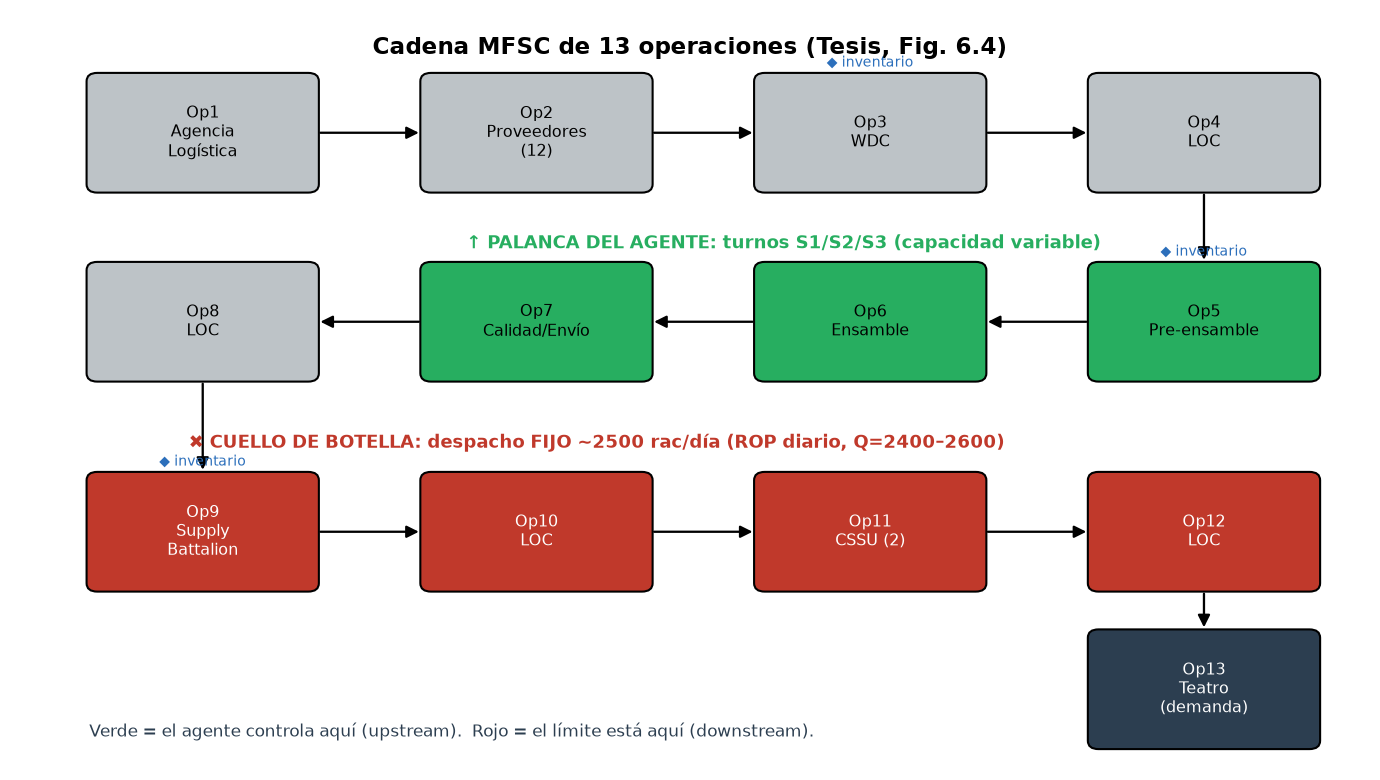
\includegraphics[width=\linewidth]{figures/figb3_chain.png}
\caption{Cadena MFSC (Tesis \cite{tesis2017}, Fig.\ 6.4). Verde: palanca del agente
(turnos, Op5--7). Rojo: cuello de botella de despacho fijo (Op9--12, $\sim$2500/día).}
\label{fig:chain}
\end{figure}

\section{La prueba: más producción NO es más entrega}
Corrimos el simulador (sin riesgos, 1 año) a S1, S2 y S3. La capacidad de ensamblaje es
$320.5$ raciones/h $\times$ \{8, 16, 24\} h/día $=$ \{2564, 5128, 7692\} raciones/día.
Pero la entrega está topada por Op9--Op12:

\begin{table}[h]\centering\small
\begin{tabular}{lccc}
\toprule
Turno & Producido (Op5--7) & \textbf{Entregado} (vía Op9--12) & Atrapado en Op9 \\
\midrule
S1 & 656k & 642k & 2{,}483 \\
S2 & 1{,}312k & \textbf{729k} & 564{,}917 \\
S3 & 1{,}969k & \textbf{729k} \ (\emph{idéntico a S2}) & \bad{1{,}212{,}917} \\
\bottomrule
\end{tabular}
\caption{S2 y S3 \textbf{entregan exactamente lo mismo} ($729$k) aunque S3 produce 50\%
más. El exceso queda atrapado en el Supply Battalion (Op9). Simulación, 1 año, sin riesgos.}
\label{tab:deliver}
\end{table}

\begin{figure}[h]\centering
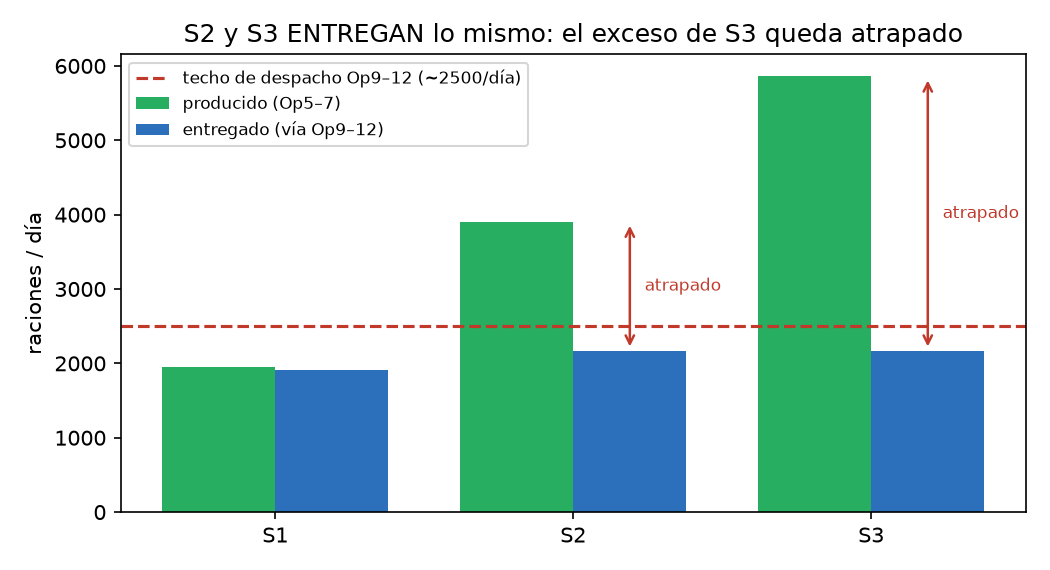
\includegraphics[width=0.72\linewidth]{figures/figb1_prod_vs_deliver.png}
\caption{La barra de ``producido'' crece con el turno, pero la de ``entregado'' se topa
en $\sim$2500/día (línea roja). Todo lo que S3 produce de más queda atrapado.}
\label{fig:deliver}
\end{figure}

\begin{figure}[h]\centering
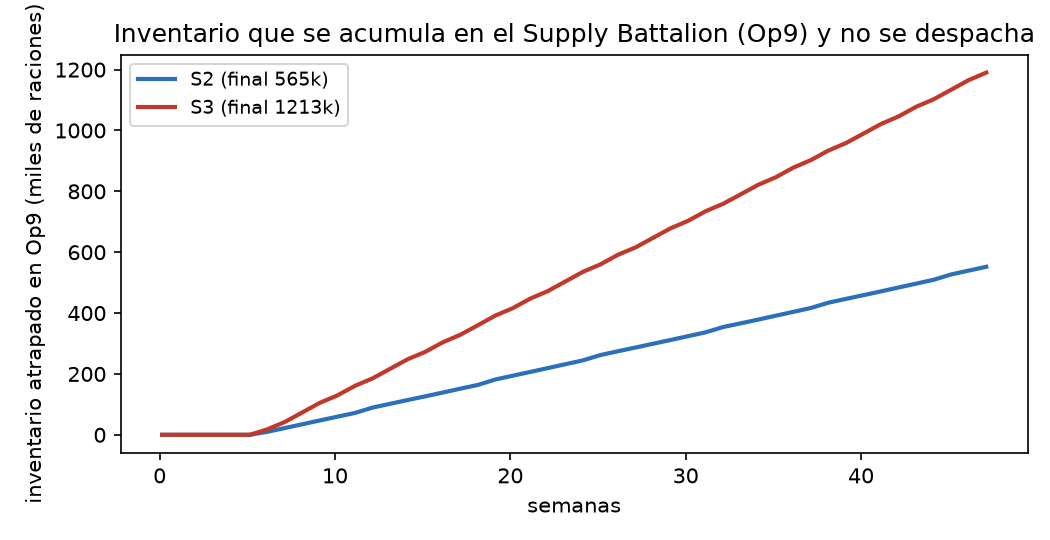
\includegraphics[width=0.72\linewidth]{figures/figb2_accumulation.png}
\caption{El inventario que el cuello de botella no despacha se acumula en Op9: bajo S3
quedan atrapadas $\sim$1.2 millones de raciones en un año.}
\label{fig:accum}
\end{figure}

\section{Por qué esto mata el aprendizaje}
La resiliencia ReT de la tesis \cite{tesis2017} incluye el \emph{fill rate}
(Eq.\ 5.4 / Fig.\ 6.5), que depende de lo \textbf{entregado}, no de lo producido
(Fig.\ \ref{fig:retlink}). Como la entrega está topada por Op9--Op12:
\begin{itemize}
  \item Subir de S1 a S2 \ok{sí} cierra el déficit de producción $\Rightarrow$ mejora ReT.
  \item Pasar de S2 a S3 \bad{no} aumenta la entrega $\Rightarrow$ no mejora ReT, solo
  acumula inventario y costo. Por eso \textbf{S2 ya es casi óptima} y cualquier RL que
  solo mueva turnos/inventario aguas arriba no tiene casi nada que ganar.
  \item El inventario tampoco ayuda: el problema no es \emph{falta de material}, es la
  \emph{tasa de despacho} de Op9--Op12, que es un parámetro fijo de la tesis.
\end{itemize}

\begin{figure}[h]\centering
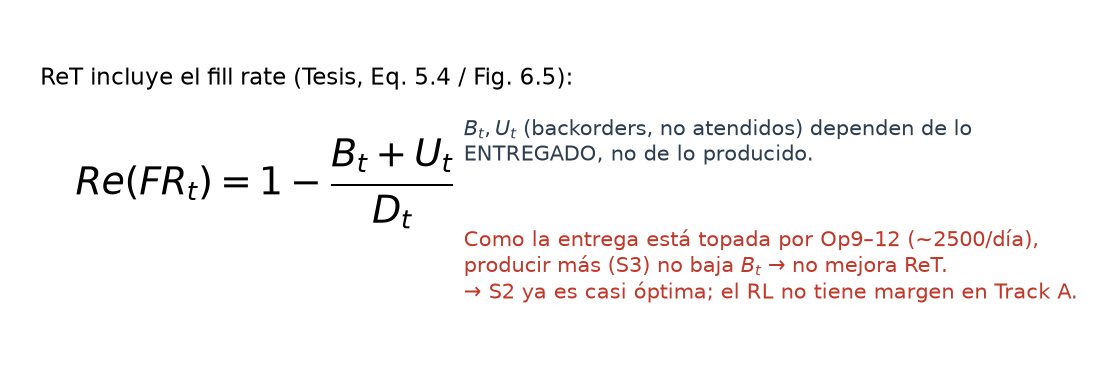
\includegraphics[width=0.86\linewidth]{figures/figb4_ret_link.png}
\caption{El fill rate (y por tanto ReT) está acotado por la entrega, no por la
producción. Producir más allá de S2 no baja los backorders $B_t$.}
\label{fig:retlink}
\end{figure}

\section{Conclusión y consecuencia para el paper}
\textbf{¿En qué operación está el problema?} En la \bad{distribución aguas abajo,
Op9--Op12} (Supply Battalion $\to$ líneas de comunicación $\to$ CSSU $\to$ MP).
\textbf{¿Por qué?} Porque despachan a un ritmo fijo ($\sim$2500 raciones/día, ROP diario)
que el agente no puede cambiar, y que ya está saturado por S2. Las palancas de decisión
de la tesis (turnos Op5--7, inventario Op3/5/9) están \emph{aguas arriba} de ese límite.

\medskip
\noindent Esto explica, con la propia estructura de la tesis, los resultados del reporte
principal: todo RL en Track A pierde contra la estática S2, porque el margen real
está \bad{donde el agente no tiene palanca}. El aprendizaje endógeno $L_{t-1}$ solo
puede cobrar valor si: (i) se le da al agente una palanca \emph{en} el cuello de botella
(controlar el despacho de Op10/Op12 --- nuestro Track B), o (ii) se introduce inercia
realista (lag y presupuesto finito de turnos) para que anticipar el régimen tenga valor.

\begin{thebibliography}{1}
\bibitem{tesis2017} Garrido-Rios. \emph{Modelo de simulación de eventos discretos para
la resiliencia de una cadena de suministro militar de alimentos (MFSC)}. Tesis, 2017.
(Fig.\ 6.4 operaciones; Tabla 6.4 demanda; Eq.\ 5.4 / Fig.\ 6.5 fill rate y ReT;
Tablas 6.16/6.20 inventario y turnos.)
\end{thebibliography}
\end{document}
